
%\begin{tcolorbox}[colframe=black, colback=red]
\section{Your Decks}
\subsection*{The Action Deck}
%Dezenter reminder über das level up mit Seitenzahl zu level up segment
The Action Deck contains all action cards you can draw and subsequently play during combat.\\
As a deckbuilding game the action deck will continue to evolve during gameplay. \textit{See Chapter \pageref{Section_CharacterBuilding}}\\

\begin{figure}[ht]
	\begin{minipage}[t][5cm][t]{0.5\textwidth}
		\begin{minipage}[t][5cm][t]{0.9\textwidth}
			\textbf{Action Cards}
			\begin{itemize}
				\item \textbf{Name} - Name of the card
				\item\textbf{Cost} - Can be mandatory, optional or none
				\item\textbf{Actions} - What the card does once played
				\item\textbf{Class/Species} - From where you obtained the card
				\item\textbf{Tier} - Strength of a card
			\end{itemize}
			%\item \textbf{Damage} - Damage and Kill
			%\item \textbf{Boons} - Buff yourself and enemies
			%\item \textbf{Banes} - Debuff the enemies
			%\item \textbf{Elements} - Create elements
			%\item \textbf{AOE} - Affect multiple enemies
			
		\end{minipage}
	\end{minipage}
	\begin{minipage}[t][5cm][t]{0.5\textwidth}
		
		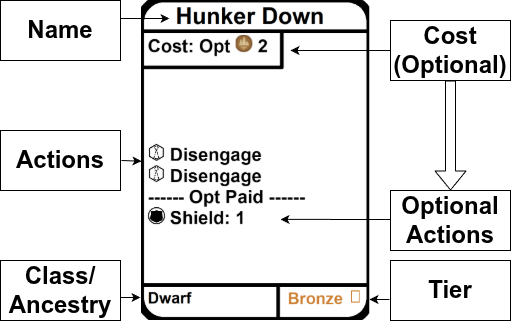
\includegraphics[width=0.9\linewidth, valign=t]{ExplanationPics/ActionCard.drawio.png}		
	\end{minipage}	
\end{figure}
%Remember: Reading the card explains the card. Except when it doesn't. In that case, check the FAQ.
\begin{tcolorbox}[colframe=black, colback=white]
	By default, your action deck will always contain 16 Cards. When a new card is added in between a fight, you must choose an old one to take out.
\end{tcolorbox}
%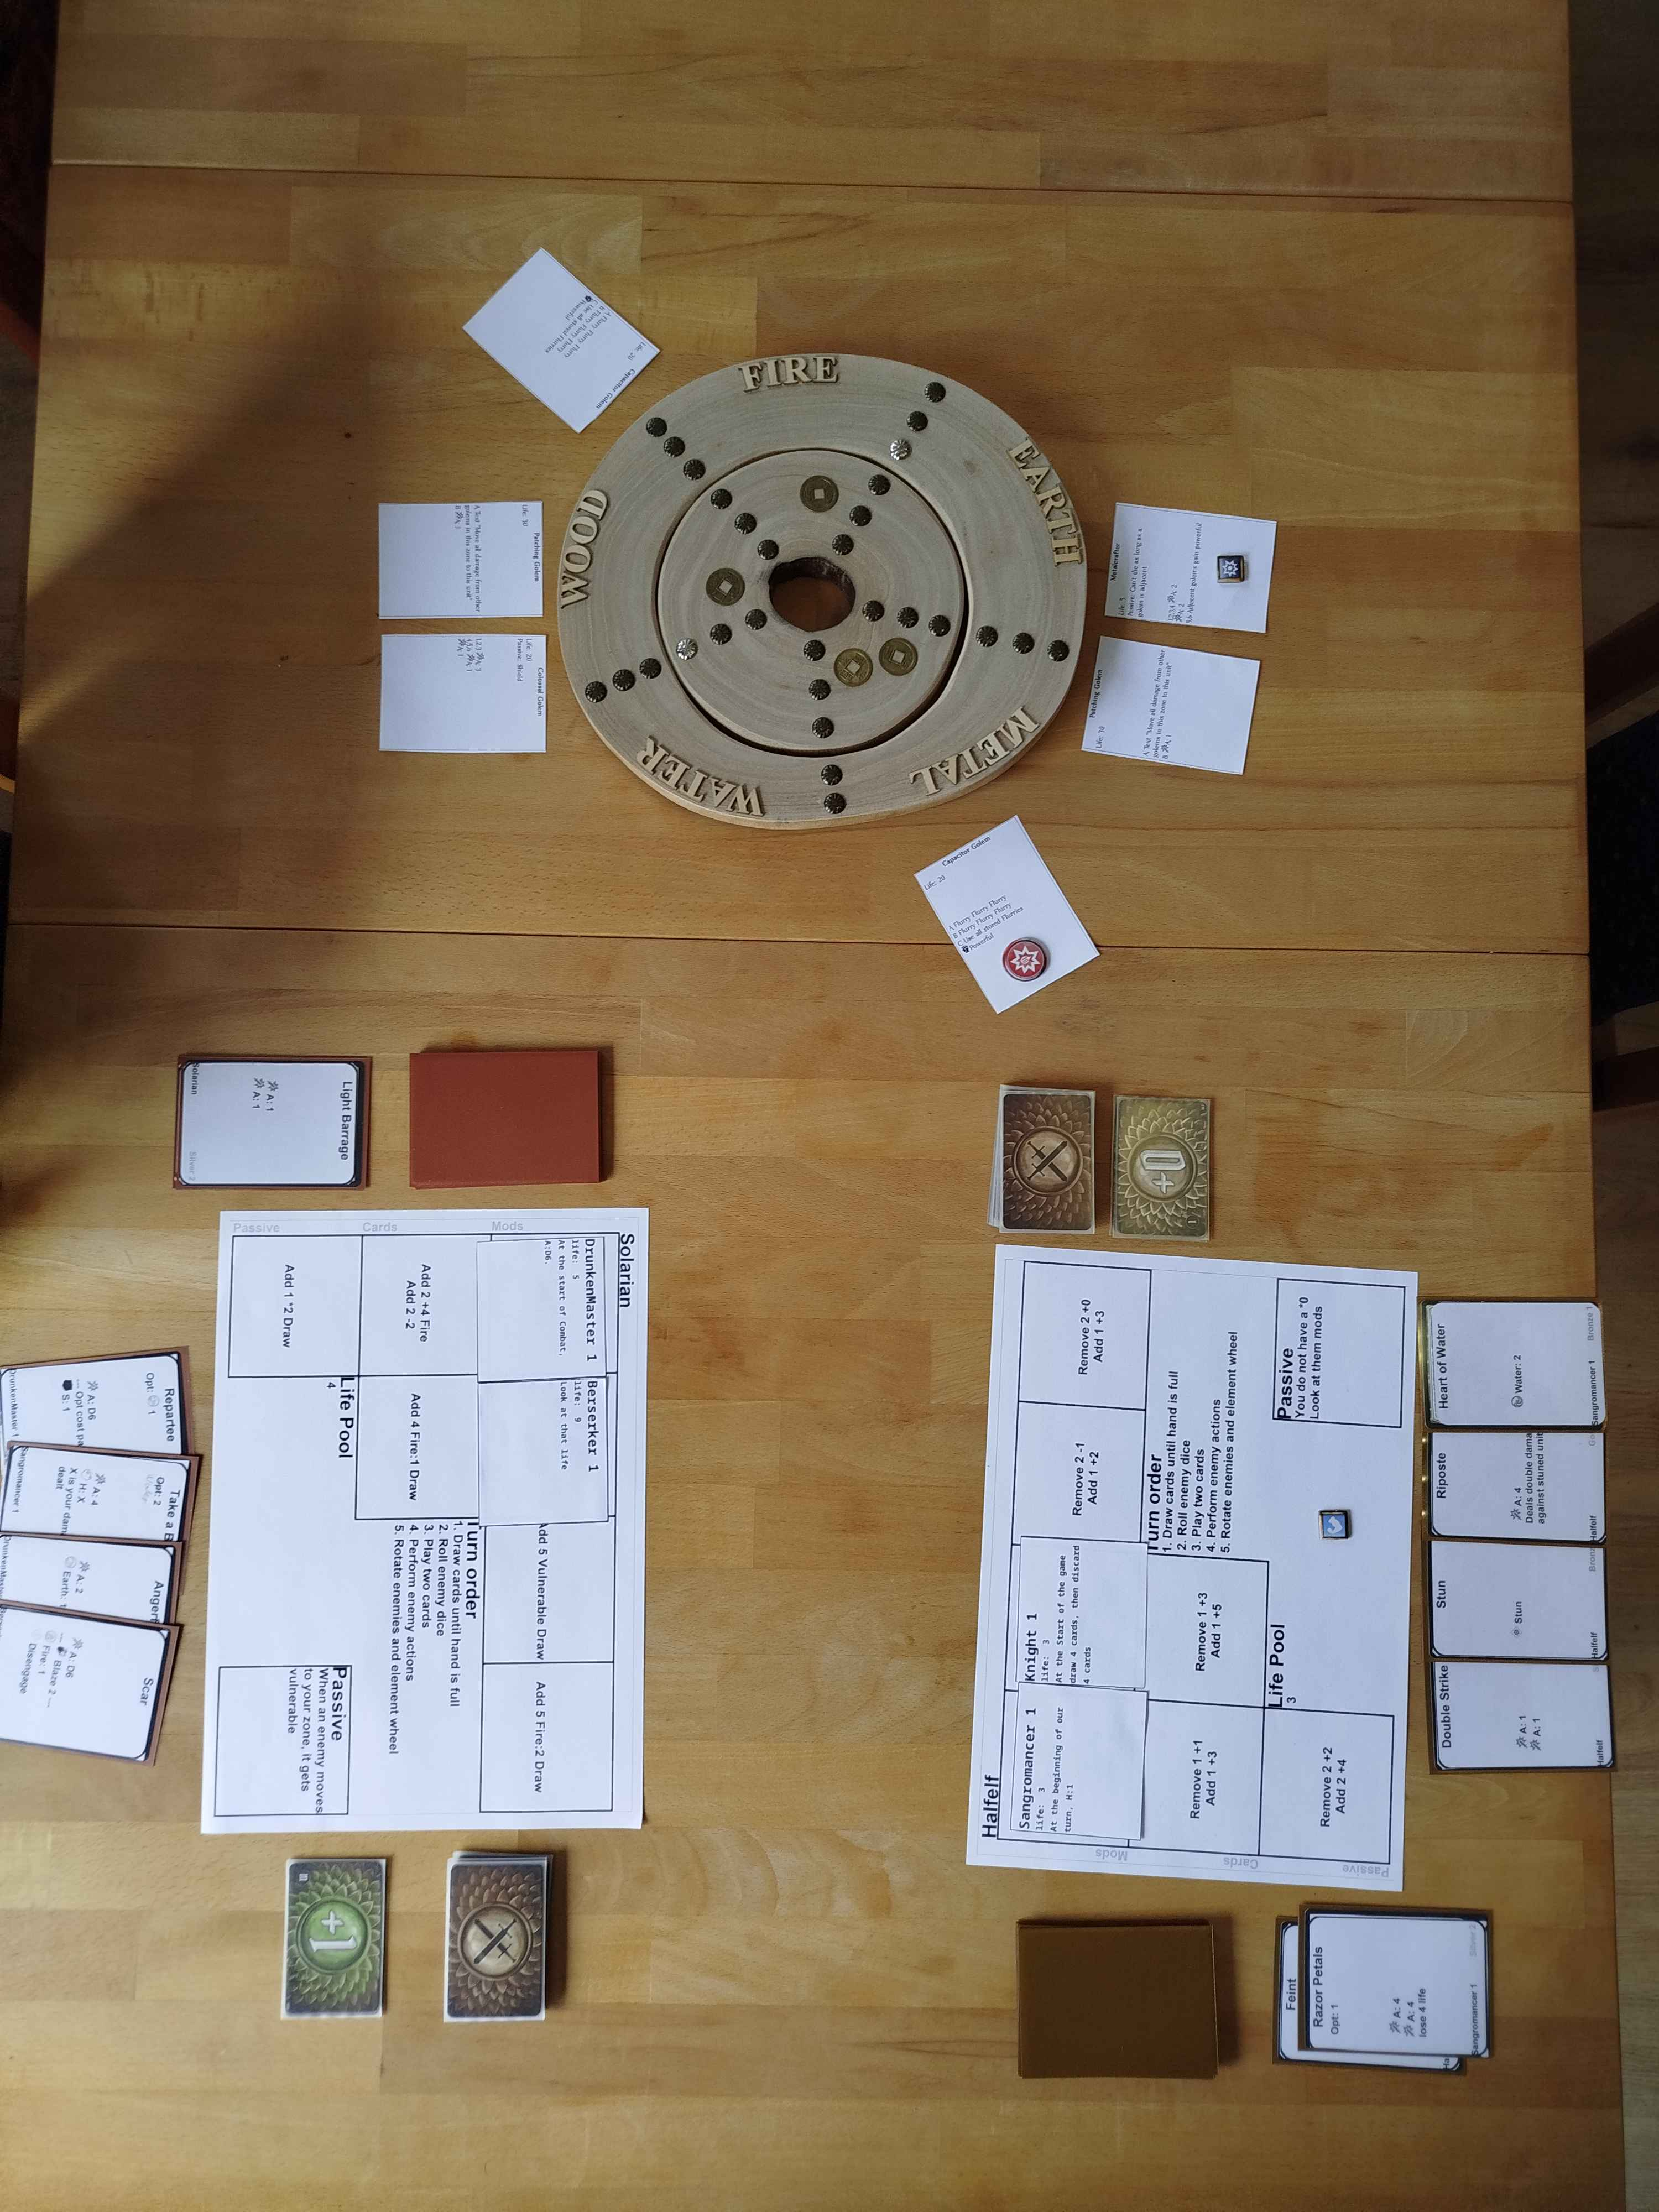
\includegraphics[width=0.8\textwidth]{ExplanationPics/TwoBoards.jpg}




\subsection*{The Ancestry Dice}
These dice modify the results of your \symAttack attacks.
Every time you pick a class, you will get an additional ancestry die. You always use all dice at once.
The ancestry dice can have four effects

\begin{figure}[ht]
	\begin{minipage}[t][5cm][t]{0.5\textwidth}
		\begin{minipage}[t][5cm][t]{0.9\textwidth}
			\begin{itemize}
				\item \textbf{Numerical} - Add or subtract damage to your \symAttack attack
				\item\textbf{Elements \symFire \symEarth \symMetal \symWater \symWood} - Always added to the wheel after the \symAttack attack
				\item\textbf{Boons} - Affect you immediately, and can help the \symAttack attack
				\item\textbf{Bane} - Affect the enemy immediately, and can help your \symAttack attack
			\end{itemize}
			%\item \textbf{Damage} - Damage and Kill
			%\item \textbf{Boons} - Buff yourself and enemies
			%\item \textbf{Banes} - Debuff the enemies
			%\item \textbf{Elements} - Create elements
			%\item \textbf{AOE} - Affect multiple enemies
			
		\end{minipage}
	\end{minipage}
	\begin{minipage}[t][5cm][t]{0.5\textwidth}
		
		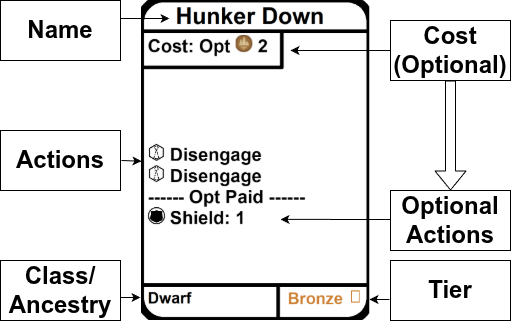
\includegraphics[width=0.9\linewidth, valign=t]{ExplanationPics/ActionCard.drawio.png}		
	\end{minipage}	
\end{figure}
\begin{tcolorbox}[colframe=black, colback=white]
	Each die also has one side with a reminder of the ancestry it belongs to
\end{tcolorbox}